

\section{Introduction}
This report outlines the design and verification of a Finite State Machine for an automated vending machine. The system features three input signals corresponding to coin insertions of 5, 10, and 25 cents. The system's outputs include a dispense signal and a 3-bit binary value representing the specific amount of change to be returned to the user.

\section{RTL Design Specification}

Before diving into the state machine logic, this section outlines the hardware interface of the Vending Machine module. The table below provides a comprehensive description of all input and output signals, including their types, bit-widths, and functional roles within the design.

\begin{table}[H]
	\centering
	
	\label{tab:signals}
	\renewcommand{\arraystretch}{1.4}
	\begin{tabularx}{\textwidth}{|l|c|c|X|}
		\hline
		\textbf{Signal Name} & \textbf{Type} & \textbf{Width} & \textbf{Description} \\ \hline
		\texttt{i\_clk} & Input & 1 & System clock for synchronous logic operations. \\ \hline
		\texttt{i\_rst\_n} & Input & 1 & Asynchronous active-low reset signal. \\ \hline
		\texttt{i\_nickle} & Input & 1 & Asserted when a 5\textcent{} coin (Nickel) is inserted. \\ \hline
		\texttt{i\_dime} & Input & 1 & Asserted when a 10\textcent{} coin (Dime) is inserted. \\ \hline
		\texttt{i\_quarter} & Input & 1 & Asserted when a 25\textcent{} coin (Quarter) is inserted[cite: 1, 5]. \\ \hline
		\texttt{o\_soda} & Output & 1 & Asserted high when a product is successfully dispensed. \\ \hline
		\texttt{o\_change[2:0]} & Output & 3 & 3-bit binary value representing the amount of change returned. \\ \hline
	\end{tabularx}
	\caption{Signal Descriptions for the Vending Machine Module}
\end{table}



\subsection{FSM Archcitecture}

\begin{figure}[H]
	\centering
	\includegraphics[width=1.0\linewidth]{figures_tech/FSM.png} 
	\caption{FSM Moore} 
	\label{fig:so_do_1}
\end{figure}


This project employs a Moore Finite State Machine (FSM) architecture due to its simplicity, ease of implementation, and widespread adoption in hardware design. The architecture follows a standard state machine topology: external inputs feed into a combinational logic block to evaluate the 'Next State'. This value is then registered by a sequential logic block, which updates the 'Present State' at each clock cycle. A defining characteristic of the Moore FSM utilized in this design is that the system outputs depend exclusively on the Present State, whereas the Next State is a function of both the Present State and the external inputs.
\newpage
\subsection{State Machine Diagram}

The following table details the transition logic of the initial 13-state FSM, covering every possible credit accumulation path before any state reduction was applied.

\begin{table}[H]
	\centering

	\label{tab:13_state_table}
	\renewcommand{\arraystretch}{1.2}
	\small
	\begin{tabular}{|c|c|c|c|}
		\hline
		\textbf{Present State} & \textbf{Input (N, D, Q)} & \textbf{Output (Soda, Change)} & \textbf{Next State} \\ \hline
		IDLE (0\textcent) & 5\textcent / 10\textcent / 25\textcent & 0 / 000 & S5 / S10 / S25 \\ \hline
		S5 (5\textcent)   & 5\textcent / 10\textcent / 25\textcent & 0 / 000 & S10 / S15 / S30 \\ \hline
		S10 (10\textcent) & 5\textcent / 10\textcent / 25\textcent & 0 / 000 & S15 / S20 / S35 \\ \hline
		S15 (15\textcent) & 5\textcent / 10\textcent / 25\textcent & 0 / 000 & S20 / S25 / S40 \\ \hline
		S20 (20\textcent) & - & 1 / 000 & IDLE \\ \hline
		S25 (25\textcent) & - & 1 / 001 & IDLE \\ \hline
		S30 (30\textcent) & - & 1 / 010 & IDLE \\ \hline
		S35 (35\textcent) & - & 1 / 011 & IDLE \\ \hline
		S40 (40\textcent) & - & 1 / 100 & IDLE \\ \hline
		% Ghi chú: Các trạng thái trung gian khác dẫn đến đích
		\multicolumn{4}{|c|}{... (Remaining intermediate transitions omitted for brevity) ...} \\ \hline
	\end{tabular}
		\caption{Original FSM State Transition Table (13 States)}
\end{table}


	
	While the 13-state model provides a comprehensive logical map, it contains redundant transitions that increase hardware overhead. To optimize resource utilization and simplify the control logic, we applied state reduction techniques to merge equivalent states, resulting in a streamlined 9-state architecture that maintains full functional compliance with the original specifications.
	\begin{table}[H]
		\centering
	
		\label{tab:9_state_table}
		\renewcommand{\arraystretch}{1.2}
		\small
		\begin{tabular}{|c|c|c|c|}
			\hline
			\textbf{Present State} & \textbf{Input (N, D, Q)} & \textbf{Output (Soda, Change)} & \textbf{Next State} \\ \hline
			IDLE & 5\textcent / 10\textcent / 25\textcent & 0 / 000 & S5 / S10 / D25 \\ \hline
			S5   & 5\textcent / 10\textcent / 25\textcent & 0 / 000 & S10 / S15 / D30 \\ \hline
			S10  & 5\textcent / 10\textcent / 25\textcent & 0 / 000 & S15 / D20 / D35 \\ \hline
			S15  & 5\textcent / 10\textcent / 25\textcent & 0 / 000 & D20 / D25 / D40 \\ \hline
			D20  & - & 1 / 000 & IDLE \\ \hline
			D25  & - & 1 / 001 & IDLE \\ \hline
			D30  & - & 1 / 010 & IDLE \\ \hline
			D35  & - & 1 / 011 & IDLE \\ \hline
			D40  & - & 1 / 100 & IDLE \\ \hline
		\end{tabular}
			\caption{Optimized FSM State Transition Table (9 States)}
		
	\end{table}
	\begin{figure}[H]
	\centering
	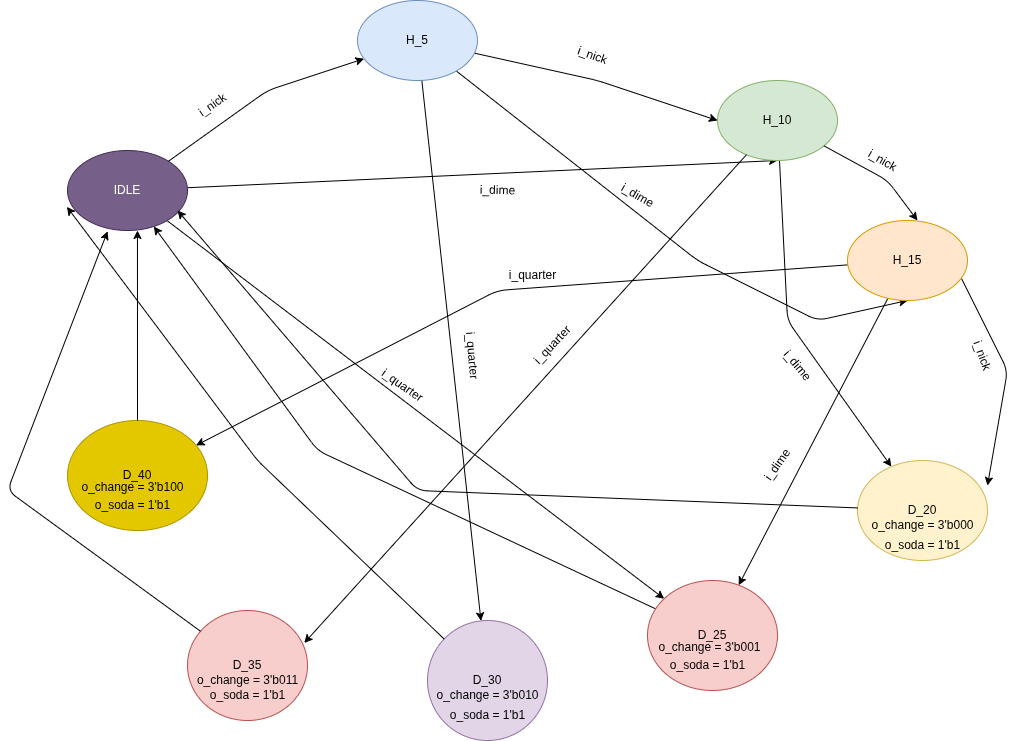
\includegraphics[width=1.0\linewidth]{figures_tech/FSM_control.png} 
	\caption{FSM Control} 
	\label{fig:so_do_1}
\end{figure}


The system accepts sequential insertions of 5¢, 10¢, and 25¢ coins. Once the accumulated value reaches or exceeds the 20¢ threshold, the FSM asserts the dispense signal and outputs the corresponding change. Notably, the state machine was optimized from an initial 13-state design down to a minimized 9-state architecture. This state reduction not only conserves hardware resources but also enhances design clarity, and it has been fully verified to comply with the functional specifications.

\section{Verification Architecture}
\begin{figure}[H]
	\centering
	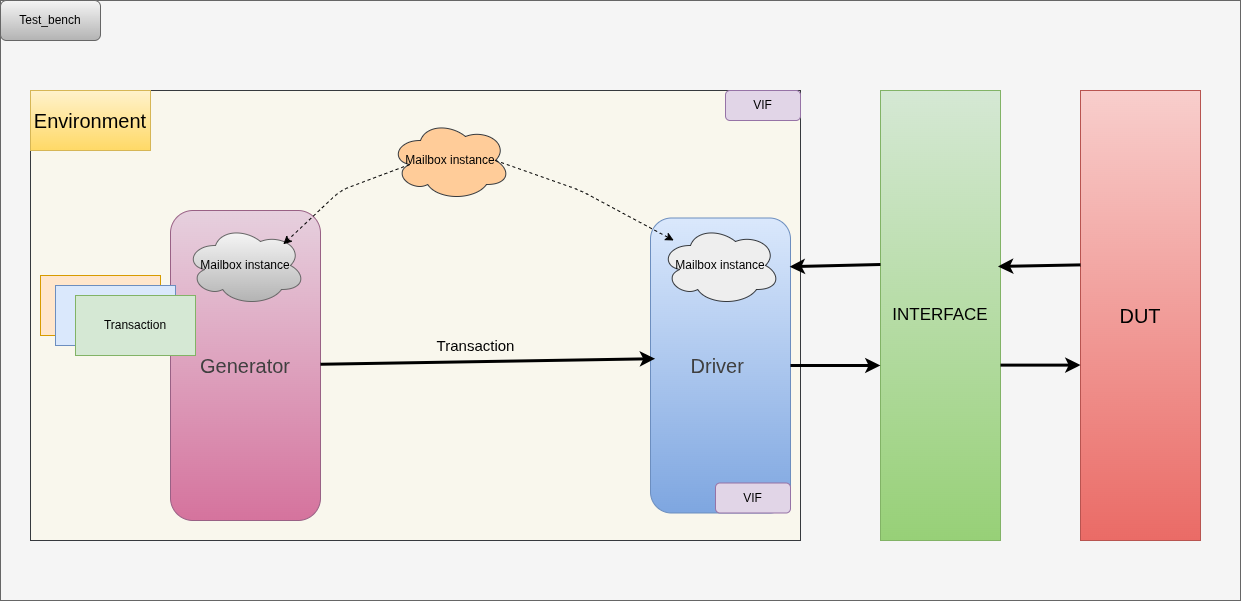
\includegraphics[width=1.0\linewidth]{figures_tech/env_tb.png} 
	\caption{FSM Control} 
	\label{fig:so_do_1}
\end{figure}


To verify this design, a reusable verification environment was developed using SystemVerilog Object-Oriented Programming (OOP) principles. The environment comprises fundamental components: Transaction, Generator, Driver, Environment, Interface, and the Device Under Test (DUT). To generate scenarios and stimulate the DUT, a handshake mechanism was implemented between the Generator and the Driver using a Mailbox, which operates as a FIFO buffer. Specifically, the Generator instantiates and packs transaction objects, then pushes them into the Mailbox. Concurrently, the Driver retrieves these transactions, translates them into pin-level logic signals, and drives the DUT via the Interface. This automated process continues until all transactions are exhausted. Finally, the functional correctness of the design is evaluated by analyzing simulation waveforms under two methodologies: Directed Testing and Constrained Random Testing.

The above diagram clearly illustrates the hierarchical structure and the handshake mechanism within the verification environment:
\begin{itemize}
	\item \textbf{Transaction:} A data class that encapsulates the coin-insertion signals.
	\item \textbf{Generator:} The block responsible for generating stimulus (supporting both directed and random scenarios) and pushing it into the Mailbox.
	\item \textbf{Driver:} The physical execution block that retrieves data from the Mailbox via a common communication port and drives the DUT's signal pins through a Virtual Interface (VIF).
	\item \textbf{DUT \& Interface:} The hardware block under test, connected to the environment via signal wires defined within the Interface.
\end{itemize}

\section{Test Scenarios \& Simulation Results}

This section evaluates the functional correctness of the Vending Machine FSM through two main testing methodologies. The simulation ensures that the design adheres to the specifications and handles various credit states reliably.

\subsection{Directed Test}
The directed test phase focuses on exhaustive state coverage, verifying every terminal state from \texttt{D\_20} to \texttt{D\_40}. Each test case validates a specific coin insertion sequence and checks if the system provides the correct dispense signal and exact change.

\begin{table}[H]
	\centering
	\small % Giảm size chữ một chút để bảng gọn hơn

	\label{tab:directed_tests}
	\renewcommand{\arraystretch}{1.5}
	% Sử dụng tabularx với chiều rộng \textwidth
	% Cột 'X' sẽ tự động giãn/co để tránh tràn lề
	\begin{tabularx}{\textwidth}{|c|X|c|c|c|c|}
		\hline
		\textbf{Case} & \textbf{Coin Sequence (Stimulus)} & \textbf{Total} & \textbf{Target} & \textbf{Change} & \textbf{Log} \\ \hline
		1 & 10\textcent{} + 10\textcent{} & 20\textcent{} & \texttt{D\_20} & 0\textcent{} (\texttt{3'b000}) & \textbf{PASSED} \\ \hline
		2 & 25\textcent{} & 25\textcent{} & \texttt{D\_25} & 5\textcent{} (\texttt{3'b001}) & \textbf{PASSED} \\ \hline
		3 & 5\textcent{} + 25\textcent{} & 30\textcent{} & \texttt{D\_30} & 10\textcent{} (\texttt{3'b010}) & \textbf{PASSED} \\ \hline
		4 & 10\textcent{} + 25\textcent{} & 35\textcent{} & \texttt{D\_35} & 15\textcent{} (\texttt{3'b011}) & \textbf{PASSED} \\ \hline
		5 & 5\textcent{} + 10\textcent{} + 25\textcent{} & 40\textcent{} & \texttt{D\_40} & 20\textcent{} (\texttt{3'b100}) & \textbf{PASSED} \\ \hline
	\end{tabularx}
		\caption{Summary of Directed Test Scenarios}
\end{table}
As detailed in Table \ref{tab:directed_tests}, five distinct scenarios were crafted to systematically evaluate every terminal state (from \texttt{D\_20} to \texttt{D\_40}). These cases act as functional boundary checks, ensuring that regardless of the coin combination used to reach or exceed the 20\textcent{} threshold, the FSM accurately asserts the dispense signal and calculates the correct change. The consistent \textbf{PASSED} results across all scenarios confirm the logical correctness of the combinational output block.
\subsubsection*{Log File}

\begin{table}[H]
	\centering
	\begin{tabular}{|p{0.95\textwidth}|}
		\hline
		\texttt{\small [TEST CASE 1] Target: 20c (State D\_20)} \\
		\texttt{\small The transaction have been drived to 0} \\
		\texttt{\small [1100] [test\_direct] N:0 D:1 Q:0} \\
		\texttt{\small Put the transaction is done} \\
		\texttt{\small [1100] [DRIVER] Driver bat dau run Mailbox...} \\
		\texttt{\small [1100] [DRIVER] Nhan duoc Trans ngau nhien: N:0 D:1 Q:0} \\
		\texttt{\small The transaction have been drived to 0} \\
		\texttt{\small [1450] [test\_direct] N:0 D:1 Q:0} \\
		\texttt{\small Put the transaction is done} \\
		\texttt{\small [1450] [DRIVER] Nhan duoc Trans ngau nhien: N:0 D:1 Q:0} \\
		\texttt{\small [1650] PASSED: Soda=1, Change=000} \\
		\texttt{\small } \\
		\texttt{\small [TEST CASE 2] Target: 25c (State D\_25)} \\
		\texttt{\small The transaction have been drived to 0} \\
		\texttt{\small [2150] [test\_direct] N:0 D:0 Q:1} \\
		\texttt{\small Put the transaction is done} \\
		\texttt{\small [2150] [DRIVER] Nhan duoc Trans ngau nhien: N:0 D:0 Q:1} \\
		\texttt{\small [2350] PASSED: Soda=1, Change=001} \\
		\texttt{\small } \\
		\texttt{\small [TEST CASE 3] Target: 30c (State D\_30)} \\
		\texttt{\small The transaction have been drived to 0} \\
		\texttt{\small [2850] [test\_direct] N:1 D:0 Q:0} \\
		\texttt{\small Put the transaction is done} \\
		\texttt{\small [2850] [DRIVER] Nhan duoc Trans ngau nhien: N:1 D:0 Q:0} \\
		\texttt{\small The transaction have been drived to 0} \\
		\texttt{\small [3250] [test\_direct] N:0 D:0 Q:1} \\
		\texttt{\small Put the transaction is done} \\
		\texttt{\small [3250] [DRIVER] Nhan duoc Trans ngau nhien: N:0 D:0 Q:1} \\
		\texttt{\small [3450] PASSED: Soda=1, Change=010} \\
		\texttt{\small } \\
		\texttt{\small ... (Remaining test cases omitted for brevity)} \\ \hline
	\end{tabular}
	\caption{Directed Test Simulation Log Output (Partial)}
	\label{tab:directed_log}
\end{table}


\newpage
\subsubsection*{Waveform Analysis}
 \begin{figure}[H]
	   \centering
	    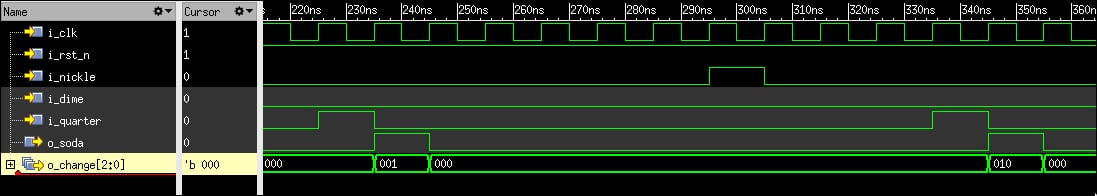
\includegraphics[width=1.0\linewidth]{figures_tech/1.jpg} 
	    \caption{Waveform Of Direct Test} % Thay bằng mô tả thực tế
	%     \label{fig:sample_image} % Nhãn để tham chiếu
	\end{figure}

As illustrated in Figure 1, the simulation waveform vividly captures a segment of the Directed Test phase, specifically demonstrating Test Case 2 and Test Case 3. In the first transaction, the assertion of the \texttt{i\_quarter} signal (25\textcent{}) immediately triggers the FSM to pull the \texttt{o\_soda} signal high and output \texttt{3'b001} (5\textcent{}) on the change bus at the next clock edge. Subsequently, the second transaction shows a sequential insertion of a nickel (\texttt{i\_nickle}) and a quarter (\texttt{i\_quarter}), accumulating to 30\textcent{}. The system correctly responds by asserting \texttt{o\_soda} and providing exactly 10\textcent{} in change (\texttt{3'b010}). This timing diagram perfectly validates the synchronous nature of the Moore FSM, proving that the outputs respond accurately without any combinational glitches.
\subsection{Constrained Random Test}

The random testing phase was executed to evaluate the FSM's robustness under unpredictable input sequences. The table below summarizes the configuration and the final verification results for this phase.

\begin{table}[H]
	\centering
	\small
	\renewcommand{\arraystretch}{1.5}
	\begin{tabularx}{\textwidth}{|l|X|}
		\hline
		\textbf{Parameter} & \textbf{Configuration / Simulation Result} \\ \hline
		\textbf{Test Methodology} & Constrained Random Verification (CRV) \\ \hline
		\textbf{Transaction Count} & 20 Automated Transactions \\ \hline
		\textbf{Randomization Rule} & One-hot coin selection ({i\_nickle, i\_dime, i\_quarter}) \\ \hline
		\textbf{Data Communication} & Mailbox-based Handshake (Synchronous FIFO) \\ \hline
		\textbf{Testing Objective} & Stress testing and exhaustive state transition coverage \\ \hline
		\textbf{Simulation Time} & 500ns (Total duration) \\ \hline
		\textbf{Final Status} & \textbf{PASSED} (100\% functional accuracy) \\ \hline
	\end{tabularx}
	\caption{Summary of Parameters and Results for the Random Test Phase}
	\label{tab:random_test_summary}
\end{table}
\newpage
To evaluate the robustness and stability of the FSM, a stress test with 20 random transactions was conducted. This phase utilizes the \texttt{randomize()} function with one-hot constraints to simulate unpredictable user behavior. The mailbox-based handshake mechanism successfully synchronized the data flow between the Generator and Driver without any data loss or logic errors.


\subsubsection*{Log File}
\begin{table}[H]
	\centering
	\begin{tabular}{|p{0.95\textwidth}|}
		\hline
		\texttt{\small [RANDOM PHASE] Running 20 random transactions...} \\
		\texttt{\small The time that We want to count is: 20} \\
		\texttt{\small [6850] [test\_random] N:1 D:0 Q:0} \\
		\texttt{\small [6850] [DRIVER] Nhan duoc Trans ngau nhien: N:1 D:0 Q:0} \\
		\texttt{\small [6860] [test\_random] N:0 D:0 Q:1} \\
		\texttt{\small [6870] [test\_random] N:0 D:0 Q:1} \\
		\texttt{\small [6880] [test\_random] N:0 D:1 Q:0} \\
		\texttt{\small [6890] [test\_random] N:0 D:1 Q:0} \\
		\texttt{\small ... (Generator continues pushing transactions into Mailbox)} \\
		\texttt{\small } \\
		\texttt{\small [7250] [DRIVER] Nhan duoc Trans ngau nhien: N:0 D:0 Q:1} \\
		\texttt{\small [7650] [DRIVER] Nhan duoc Trans ngau nhien: N:0 D:0 Q:1} \\
		\texttt{\small [8050] [DRIVER] Nhan duoc Trans ngau nhien: N:0 D:1 Q:0} \\
		\texttt{\small [8450] [DRIVER] Nhan duoc Trans ngau nhien: N:0 D:1 Q:0} \\
		\texttt{\small ... (Driver continuously popping transactions from Mailbox)} \\
		\texttt{\small } \\
		\texttt{\small [14050] [DRIVER] Nhan duoc Trans ngau nhien: N:1 D:0 Q:0} \\
		\texttt{\small [14450] [DRIVER] Nhan duoc Trans ngau nhien: N:1 D:0 Q:0} \\
		\texttt{\small } \\
		\texttt{\small --- SIMULATION FINISHED ---} \\
		\texttt{\small Simulation complete via \$finish(1) at time 1495 NS + 1} \\ \hline
	\end{tabular}
	\caption{Constrained Random Test Simulation Log Output (Partial)}
	\label{tab:random_log}
\end{table}
\newpage

\subsubsection*{Waveform Analysis}

\begin{figure}[H]
	\centering
	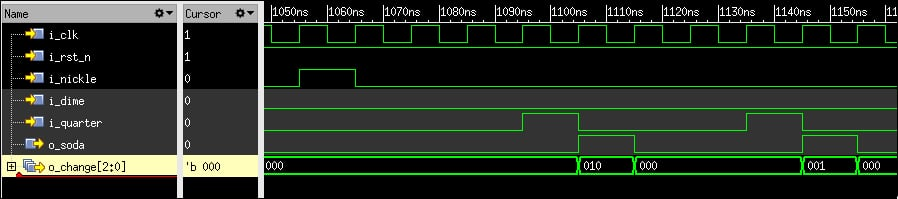
\includegraphics[width=1.0\linewidth]{figures_tech/2.jpg} 
	\caption{Waveform Of Random Test} % Thay bằng mô tả thực tế
	%     \label{fig:sample_image} % Nhãn để tham chiếu
\end{figure}

As depicted in Figure 2, the waveform captures a dynamic segment of the Constrained Random Test phase, highlighting the FSM's reliability under unpredictable input streams. In the observed time frame, the testbench randomly generates an \texttt{i\_nickle} (5\textcent) followed by an \texttt{i\_quarter} (25\textcent). The system accurately accumulates this arbitrary combination to 30\textcent, synchronously asserting the \texttt{o\_soda} signal and dispensing exactly 10\textcent{} in change (\texttt{3'b010}). Immediately following this cycle, another random transaction injects a single quarter. The FSM seamlessly processes this independent 25\textcent{} input, pulling \texttt{o\_soda} high again and outputting \texttt{3'b001} (5\textcent) on the change bus. This timing diagram confirms the design's robustness, proving that the Mailbox-driven random stimuli are processed flawlessly with strict adherence to the Moore FSM synchronous timing constraints.


\section{Conclusion}
Through this project, we have significantly improved our RTL coding skills and deepened our collective understanding of Finite State Machine (FSM) architectures, enabling us to approach similar hardware design problems with greater confidence. Most notably, this lab provided our team with valuable hands-on experience in developing a reusable Object-Oriented Programming (OOP) verification environment using SystemVerilog, which proved to be a highly effective methodology for fundamental design verification. Ultimately, the comprehensive simulation results from both directed and random test phases confirm that the Vending Machine design strictly adheres to the functional specifications and the project has been successfully completed.